% ------------------------------------------------------------------------------
%
% PREAMBLE
%
% ------------------------------------------------------------------------------

\documentclass[12pt, titlepage]{article}


\usepackage{graphicx, amsmath, amssymb, natbib, setspace, sectsty, verbatim, 
		mathrsfs, float}
\usepackage{MnSymbol}
\usepackage{multirow}
\usepackage{bm}
\usepackage[usenames, dvipsnames]{color}
\bibpunct{(}{)}{;}{a}{}{,}
\setlength{\parindent}{3em}
%\parskip = 1.5ex
%\linespread{1.3}
%\onehalfspacing

\pdfpagewidth 8.5in
\pdfpageheight 11in
\setlength{\oddsidemargin}{0.0in} \setlength{\textwidth}{6.5in}
\setlength{\topmargin}{0.15in} \setlength{\textheight}{8.5in}
\setlength{\headheight}{0.0in} \setlength{\headsep}{0.0in}

\usepackage{/mnt/ExtraDrive1/Work/shTex/mymacros}

\providecommand{\norm}[1]{\lVert#1\rVert}
\newcommand{\csection}[1]{\section[#1]{\centering #1 }}
\subsectionfont{\small}
\newcommand{\cye}[1]{\color{yellow!70!black}#1}
\newcommand{\cre}[1]{\color{red!70!black}#1}
\newcommand{\cbl}[1]{\color{blue!70!black}#1}
\newcommand{\cgr}[1]{\color{green!70!black}#1}


% ------------------------------------------------------------------------------
%
% BEGIN DOCUMENT
%
% ------------------------------------------------------------------------------

\begin{document}

\setcounter{equation}{0}
\renewcommand{\theequation}{R.\arabic{equation}}


% ------------------------------------------------------------------------------
%
%                    Section 9.10.2
%                    The wet sulfate desposition data
%
% ------------------------------------------------------------------------------


{\large \flushleft \textbf{9.10.2 Prediction of wet sulfate deposition}}

\vspace{.3cm}

We continue with our analysis from Section 8.8.3 of the clean wet sulfate deposition data in the conterminous U.S.  Our ultimate goal will be to create a map, with prediction intervals, on a grid of prediction locations across the whole U.S. that will help us assess the spatial patterns in wet sulfate deposition along with our confidence in those predictions.  We left some model selection choices open from Section 8.8.3 because predictive ability of those models will help in our selection process.  We will complete the analysis here, and begin with leave-one-out cross-validation (LOOCV).

LOOCV eliminates one datum at a time, using all of the rest of the data to predict the one that was removed.  There is a fast and a slow way to do this.  The slow way is to remove a datum and then re-estimate all of the parameters using ML or REML estimation each time.  However, with the removal of but a single datum, the parameter estimates change very little.  A fast way to achieve LOOCV is based on holding all parameters at their values as estimated by using all of the data, and then using results from partitioned matrices so that we only have to invert the covariance matrix once (which can be saved from the ML or REML estimation, so there is in fact no additional matrix inverses are required).  Recall from Section 5.6 that,
if a matrix is partitioned as,
$$
    \boldsymbol{\Sigma} = 
    \begin{bmatrix}
       \boldsymbol{\Sigma}_{11} & \boldsymbol{\Sigma}_{12} \\
       \boldsymbol{\Sigma}_{21} & \boldsymbol{\Sigma}_{22}
    \end{bmatrix}  \ \textrm{ and } \  
    \bSigma^{-1} = 
    \begin{bmatrix}
       \boldsymbol{\Sigma}^{11} & \boldsymbol{\Sigma}^{12} \\
       \boldsymbol{\Sigma}^{21} & \boldsymbol{\Sigma}^{22}
    \end{bmatrix}, 
$$
then 
$$
    \boldsymbol{\Sigma}_{11}^{-1} = \boldsymbol{\Sigma}^{11} - \boldsymbol{\Sigma}^{12} (\boldsymbol{\Sigma}^{22})^{-1} \boldsymbol{\Sigma}^{21}.
$$
Moreover, let us order the data such that the datum to be removed is last, so that $\boldsymbol{\Sigma}^{22}$ is a scalar, then the inverse of $\boldsymbol{\Sigma}^{22}$ is trivial and $\bSigma_{11} \upi$ can be computed rapidly. The main computational expense of kriging predictions rely on the inverse covariance matrix for the observed data, but in LOOCV that is given by $\bSigma_{11} \upi$, which is computed rapidly without any further matrix inverses if we already have $\bSigma \upi$. The only other quantity from $\boldsymbol{\Sigma}$ needed for prediction is the vector $\boldsymbol{\Sigma}_{12}$.  Conceptually, we just re-order the data, one at a time, putting the one to be removed last in the covariance matrices above, and that allows the predictions to be computed quickly.

Let $\hat{y}_{i} = \bar{u}$ from (9.2) be the $i$th predicted value using LOOCV where the $i$th datum has been removed, and let $\hat{v}_{i} = \sqrt{\var(\bar{u} - u)}$ from (9.3) be the $i$ prediction standard error.  Then we will consider two metrics to assess model performance.  One is the root-mean-squared prediction error (RMSPE), which we computed as
$$
\sqrt{\frac{1}{n}\sum_{i=1}^{n} (\hat{y}_{i} - y_{i})^{2} }.
$$
Models with lower RMSPE have better predictive performance.  The other metric is the 90\% prediction interval coverage, PIC90, which we computed as
$$
\frac{1}{n} \sum_{i=1}^{n} \mathcal{I}(\hat{y}_{i} - z_{1-\alpha/2}v_{i} \le y_{i} \le \hat{y}_{i} + z_{1-\alpha/2}v_{i}),
$$
where $\mathcal{I}(\cdot)$ is an indicator function, equal to 1 if its argument is true, and 0 otherwise, and $z_{1-\alpha/2}$ is a standard normal value below which contains $1-\alpha/2$ of the probability density.  We chose $\alpha = 0.1$ for PIC90, resulting in the familiar $z_{0.95} = 1.645$.

One problem with LOOCV is that it may be overly optimistic in assessing actual prediction.  A simple thought experiment reveals why.  Suppose 99 data locations were clustered very closely together, and another was separated from the cluster.  Then, for LOOCV, as we removed each datum from the cluster, we would have many nearby locations and get very precise predictions with small prediction standard errors, and they would swamp RMSPE and PIC90 if our overall goal was to predict in a region that was substantially larger than that enclosing the cluster of locations. The same is essentially true if all locations were pairs of locations that were very close to each other, but the pairs were scattered.  Still, under normal sampling scenarios, it can be a good way to evaluate models as they are all operating under the same sampling scheme.

A second way to use cross-validation is called $n$-fold cross-validation.  Here we divide the data into $n$ groups, and remove one whole group to be predicted -- this is often called the \textit{test} dataset.  The remaining data are called the \textit{training} dataset, and are used to fit a model and make predictions at the locations of the test dataset.  Then, the predictions at the locations for the test dataset can be compared to the actual values that were removed.  In fact, RMSPE and PIC90 can be computed for $n$-fold cross-validation in exactly the same way as for LOOCV, and to distinguish them, we use RMSPE$_{\textrm{Lo}}$ and PIC90$_{\textrm{Lo}}$ for LOOCV, and RMSPE$_{\textrm{Nf}}$ and PIC90$_{\textrm{Nf}}$ for $n$-fold cross-validation. With $n$-fold cross-validation we do not have to fit the model as many times, so we completely re-fit the model for each group that is removed.  Groups are often created randomly, and we will do it this way too.  If we want to get the best feel how well a model will interpolate, that includes even a bit of extrapolation at the edges, it is desirable to have just a few groups.  This may be more pessimistic about model performance than the real data because we are decreasing our sample sizes substantially.  Nevertheless, to examine both extremes, where LOOCV is overly optimistic, we used 3-fold cross-validation, which is overly pessimistic.  Because we created 3 groups randomly, we would like to ensure that our results do not depend too much on any particular randomized grouping.  Hence, we do 3-fold cross-validation 10 times, and average the results for RMSPE (by first averaging the mean-squared prediction error, and then taking the square root) and PIC90.

To further evaluate the models from from Section 8.8.3, we will consider LOOCV and 3-fold crossvalidation for polynomials with orders up to 5, again using the exponential autocovariance model.  RMSPE using LOOCV for the independence models generally goes down with increasing order of the polynomial surface (Figure~\ref{Fig:SO4_crossval}A), suggesting, like AIC and BIC, that among this set of models, a 4th or 5th order polynomial is best.  However, when it comes to predictive performance, the spatial models are much superior, having average deviations from true values of around 0.47 for lower order polynomials, versus approximately 0.53 for the higher order polynomials of the independence models, which translates to prediction intervals that are over 11\% shorter.  The problem of over-fitting polynomials is revealed more clearly by 3-fold cross-validation (Figure~\ref{Fig:SO4_crossval}C), where the RMSPE begins to increase rapidly for the independence models for the 5th order polynomial, and increases throughout for the spatial models. It also appears that for the spatial models in both Figure~\ref{Fig:SO4_crossval}A,C that REMLE is just slightly better than MLE.

\begin{figure}[H]
  \begin{center}
	    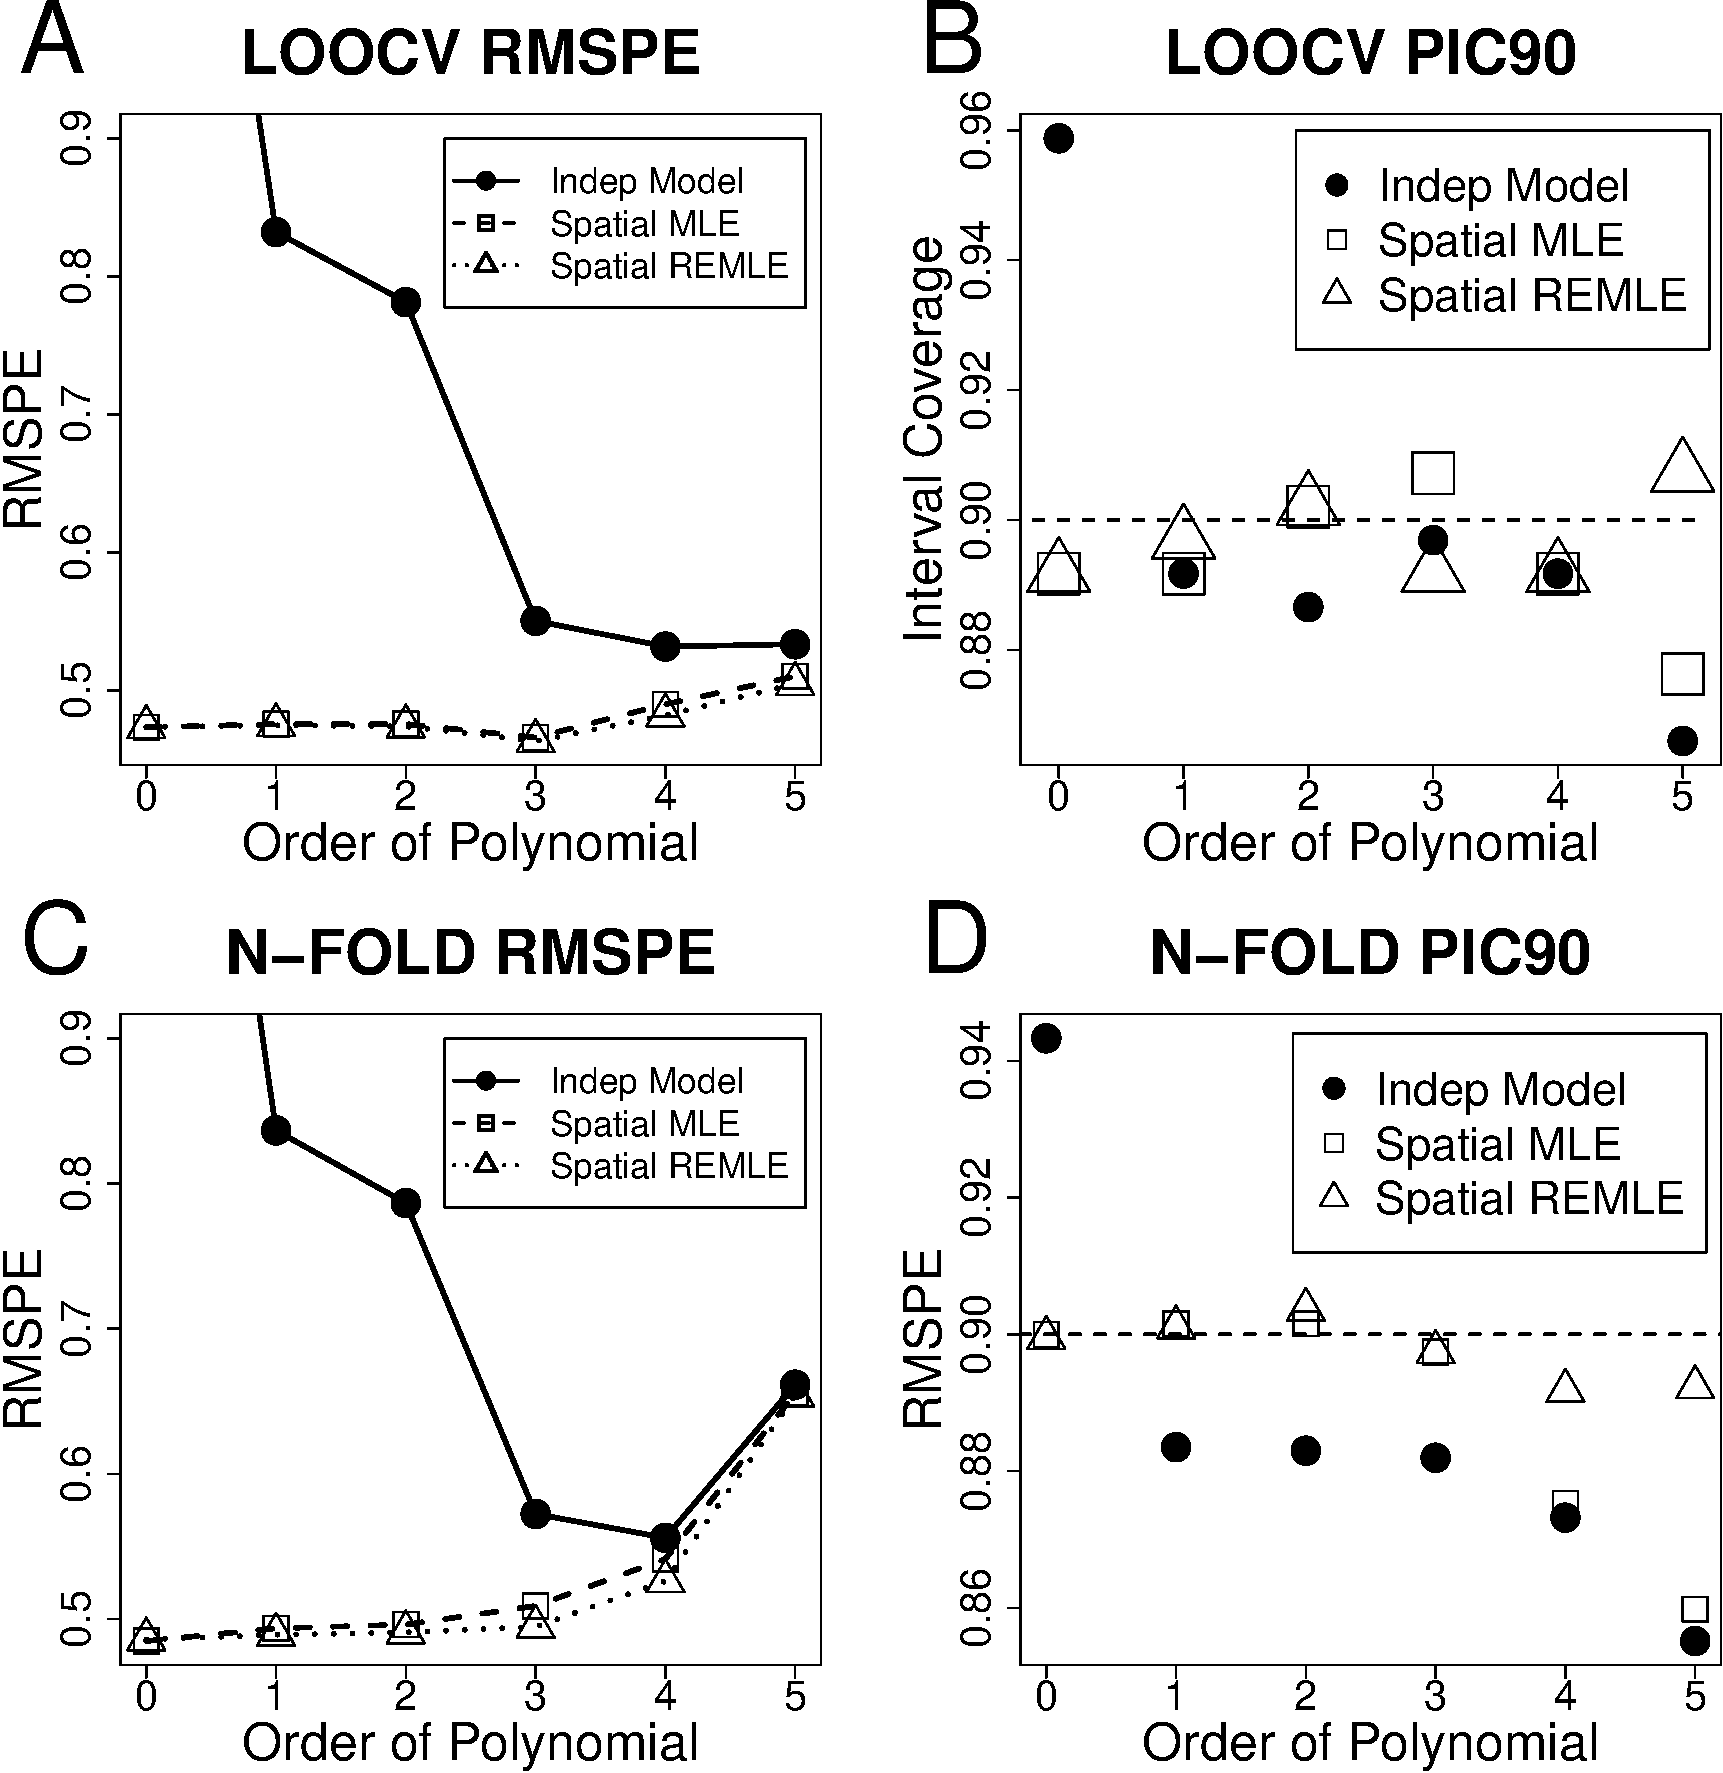
\includegraphics[width=.8\linewidth]{SO4_crossval}
  \end{center}
  \caption{Root-mean-squared prediction error (RMSPE) and 90\% prediction intervals coveraga (PIC90) using leave-one-out cross-validation (LOOCV) and 3-fold cross-validation for up to 5th order polynomial surfaces using the clean wet sulfate deposition data.  The spatial models were fit with an exponential autocovariate model using both MLE and REMLE. A. LOOCV RMSPE B. LOOCV PIC90 C. 3-fold RMSPE, and D. 3-fold PIC90. \label{Fig:SO4_crossval}}
\end{figure}

We want our prediction surfaces to be as precise as possible, but we also need to evaluate whether the estimated prediction standard-errors are valid.  By valid, we mean that a 90\% prediction interval should contain the true value 90\% of the time. For the independence models, that is approximately true for polynomial surfaces with orders 1 through 4, but the constant mean model is overly conservative (intervals that are larger than needed and thus containing the true values almost 96\% of the time, Figure~\ref{Fig:SO4_crossval}B, and 94\%, Figure~\ref{Fig:SO4_crossval}D), while the 5th order polynomial is overly optimistic (intervals that are too short and only contain the true value around 86\% of the time (Figure~\ref{Fig:SO4_crossval}B,D). The REML estimates are very close to the nominal value for all orders of the polynomial surface, while the ML estimates start to become too optimistic at order 4 using 3-fold cross-validation (Figure~\ref{Fig:SO4_crossval}D) and order 5 using LOOCV (Figure~\ref{Fig:SO4_crossval}B).

For the spatial models, based on BIC, LOOCV, and 3-fold cross-validation, there appears to be little reason to go beyond ordinary kriging.  However, we still need to choose an autocovariance model.  We fit most of the models in Table 6.1 using \texttt{spmodel}, and computed all of the model selection metrics discussed so far (Table~\ref{tab:ModelSelAutocov}).  With the exception of a few models like wave and J-Bessel, all models performed similarly. Also note that with a constant mean model, there was very little difference between LOOCV and 3-fold cross-validation. The spherical model is just slightly better than most others based on AIC, BIC, and RMSPE.  It also appears to have appropriate prediction interval coverage, so we will choose the spherical model for further analyses.
\begin{table}[h] 
				\caption{Performance metrics for various covariance functions used with a constant mean model fit with REMLE for the clean wet sulfate data. \label{tab:ModelSelAutocov}}
\begin{center}
\begin{tabular}{c|rrrrrrr}
  \hline
  \hline
  Model & m2LL & AIC & BIC & RMSPE$_{\textrm{Lo}}$ & RMSPE$_{\textrm{Nf}}$ & PIC90$_{\textrm{Lo}}$ & PIC90$_{\textrm{Nf}}$ \\
	\hline
  \hline
exponential & 302.4 & 308.4 & 318.2 & 0.473 & 0.473 & 0.892 & 0.907 \\ 
  spherical & 298.8 & 304.8 & 314.6 & 0.469 & 0.470 & 0.887 & 0.902 \\ 
  gaussian & 308.5 & 314.5 & 324.3 & 0.487 & 0.490 & 0.871 & 0.907 \\ 
  circular & 302.6 & 308.6 & 318.4 & 0.474 & 0.480 & 0.892 & 0.897 \\ 
  pentaspherical & 299.5 & 305.5 & 315.3 & 0.470 & 0.470 & 0.887 & 0.902 \\ 
  wave & 323.4 & 329.4 & 339.2 & 0.510 & 0.515 & 0.902 & 0.892 \\ 
  jbessel & 328.9 & 334.9 & 344.7 & 0.530 & 0.527 & 0.902 & 0.892 \\ 
  gravity & 301.2 & 307.2 & 317.0 & 0.477 & 0.479 & 0.887 & 0.892 \\ 
  rquad & 302.1 & 308.1 & 317.9 & 0.478 & 0.480 & 0.881 & 0.897 \\ 
  magnetic & 303.0 & 309.0 & 318.8 & 0.479 & 0.481 & 0.876 & 0.897 \\ 
  matern & 303.9 & 311.9 & 324.9 & 0.481 & 0.483 & 0.871 & 0.897 \\ 
  cauchy & 300.4 & 308.4 & 321.5 & 0.475 & 0.481 & 0.887 & 0.892 \\ 
  pexponential & 298.3 & 306.3 & 319.4 & 0.473 & 0.471 & 0.887 & 0.902 \\
   \hline
	\hline
\end{tabular}
\end{center}
\end{table}

Now we are ready to make maps of wet sulfate deposition across the U.S.  We created an evenly spaced grid of points and clipped them to the boundaries of the continental U.S., resulting in 3663 prediction locations.  We used 5 different models to illustrate various features of the resulting maps. Figure~\ref{Fig:SO4_predMaps}A shows predictions for a 4th order polynomial assuming independent errors. The prediction standard errors show the typical pattern for regression models, where the variance is smallest near the mean of the explanatory variables (spatial coordinates in this case).  Hence, the prediction standard errors are smallest near the center of the country, somewhat weighted by the fact that there are more samples in the northeast (Figure~\ref{Fig:SO4_predMaps}B). For this 4th order polynomial model, standard errors are marginally reliable, as shown by PIC90 from LOOCV and 3-fold cross-validations. 

The spatial model with a constant mean and a spherical autocovariance is a more flexible surface than the polynomial surface (Figure~\ref{Fig:SO4_predMaps}C).  For example, there is a small area of higher sulfate deposition along the middle southern boarder of the U.S. near New Orleans, in the state of Louisiana, which is shaped like a boot. The higher concentrations are apparent in the ``toe'' of the boot.  An autocorrelated surface is more flexible to take on smaller fluctuations like this.  The map of prediction standard errors (Figure~\ref{Fig:SO4_predMaps}D) exhibits a ``bull's eye'' pattern around locations with observed data, which is characteristic of many of the autocovariance models, this map is very different then the smooth surface in Figure~\ref{Fig:SO4_predMaps}B.  Overall, the estimated prediction standard errors in Figure~\ref{Fig:SO4_predMaps}D are significantly lower than those of Figure~\ref{Fig:SO4_predMaps}B, which we we believe to be valid based on our cross-validation analysis of these data. 

We also show that, while we chose the spherical model, many of the other covariance functions would give very similar results (e.g., the exponential model in Figures~\ref{Fig:SO4_predMaps}E,F. There is some advice in the literature suggesting that the choice of which autocovariance function is not that important, at least not in comparison to the important choice a spatial model versus the model assuming independent errors.  To a certain extent, this is even true for these data when comparing the spherical model with a constant mean (Figures~\ref{Fig:SO4_predMaps}C,D) to a spherical model with a 3rd-order polynomial on the coordinates as fixed effects (Figures~\ref{Fig:SO4_predMaps}G,H), where the prediction standard errors are somewhat more diffuse, but the prediction maps are virtually identical.

However, we suggest that for a practical analysis several models should be tried to see if and where they differ.  One model that is often very different from the others is the Gaussian autocovariance model.  It creates very smooth surfaces, and Figure~\ref{Fig:SO4_predMaps}I shows that the area of higher concentration in the toe of Louisiana (Figure~\ref{Fig:SO4_predMaps}C,E,G) is not apparent when using this model, and the prediction standard errors change more gradually (Figure~\ref{Fig:SO4_predMaps}J), rather than having the bull's eye effect.  Generally, autocovariance models that are flat near the origin, and having a sigmoid shape, will behave more like Figures~\ref{Fig:SO4_predMaps}I,J, while those that drop rapidly and linearly near the origin will behave more like Figures~\ref{Fig:SO4_predMaps}C,D.

\begin{figure}[H]
  \begin{center}
	    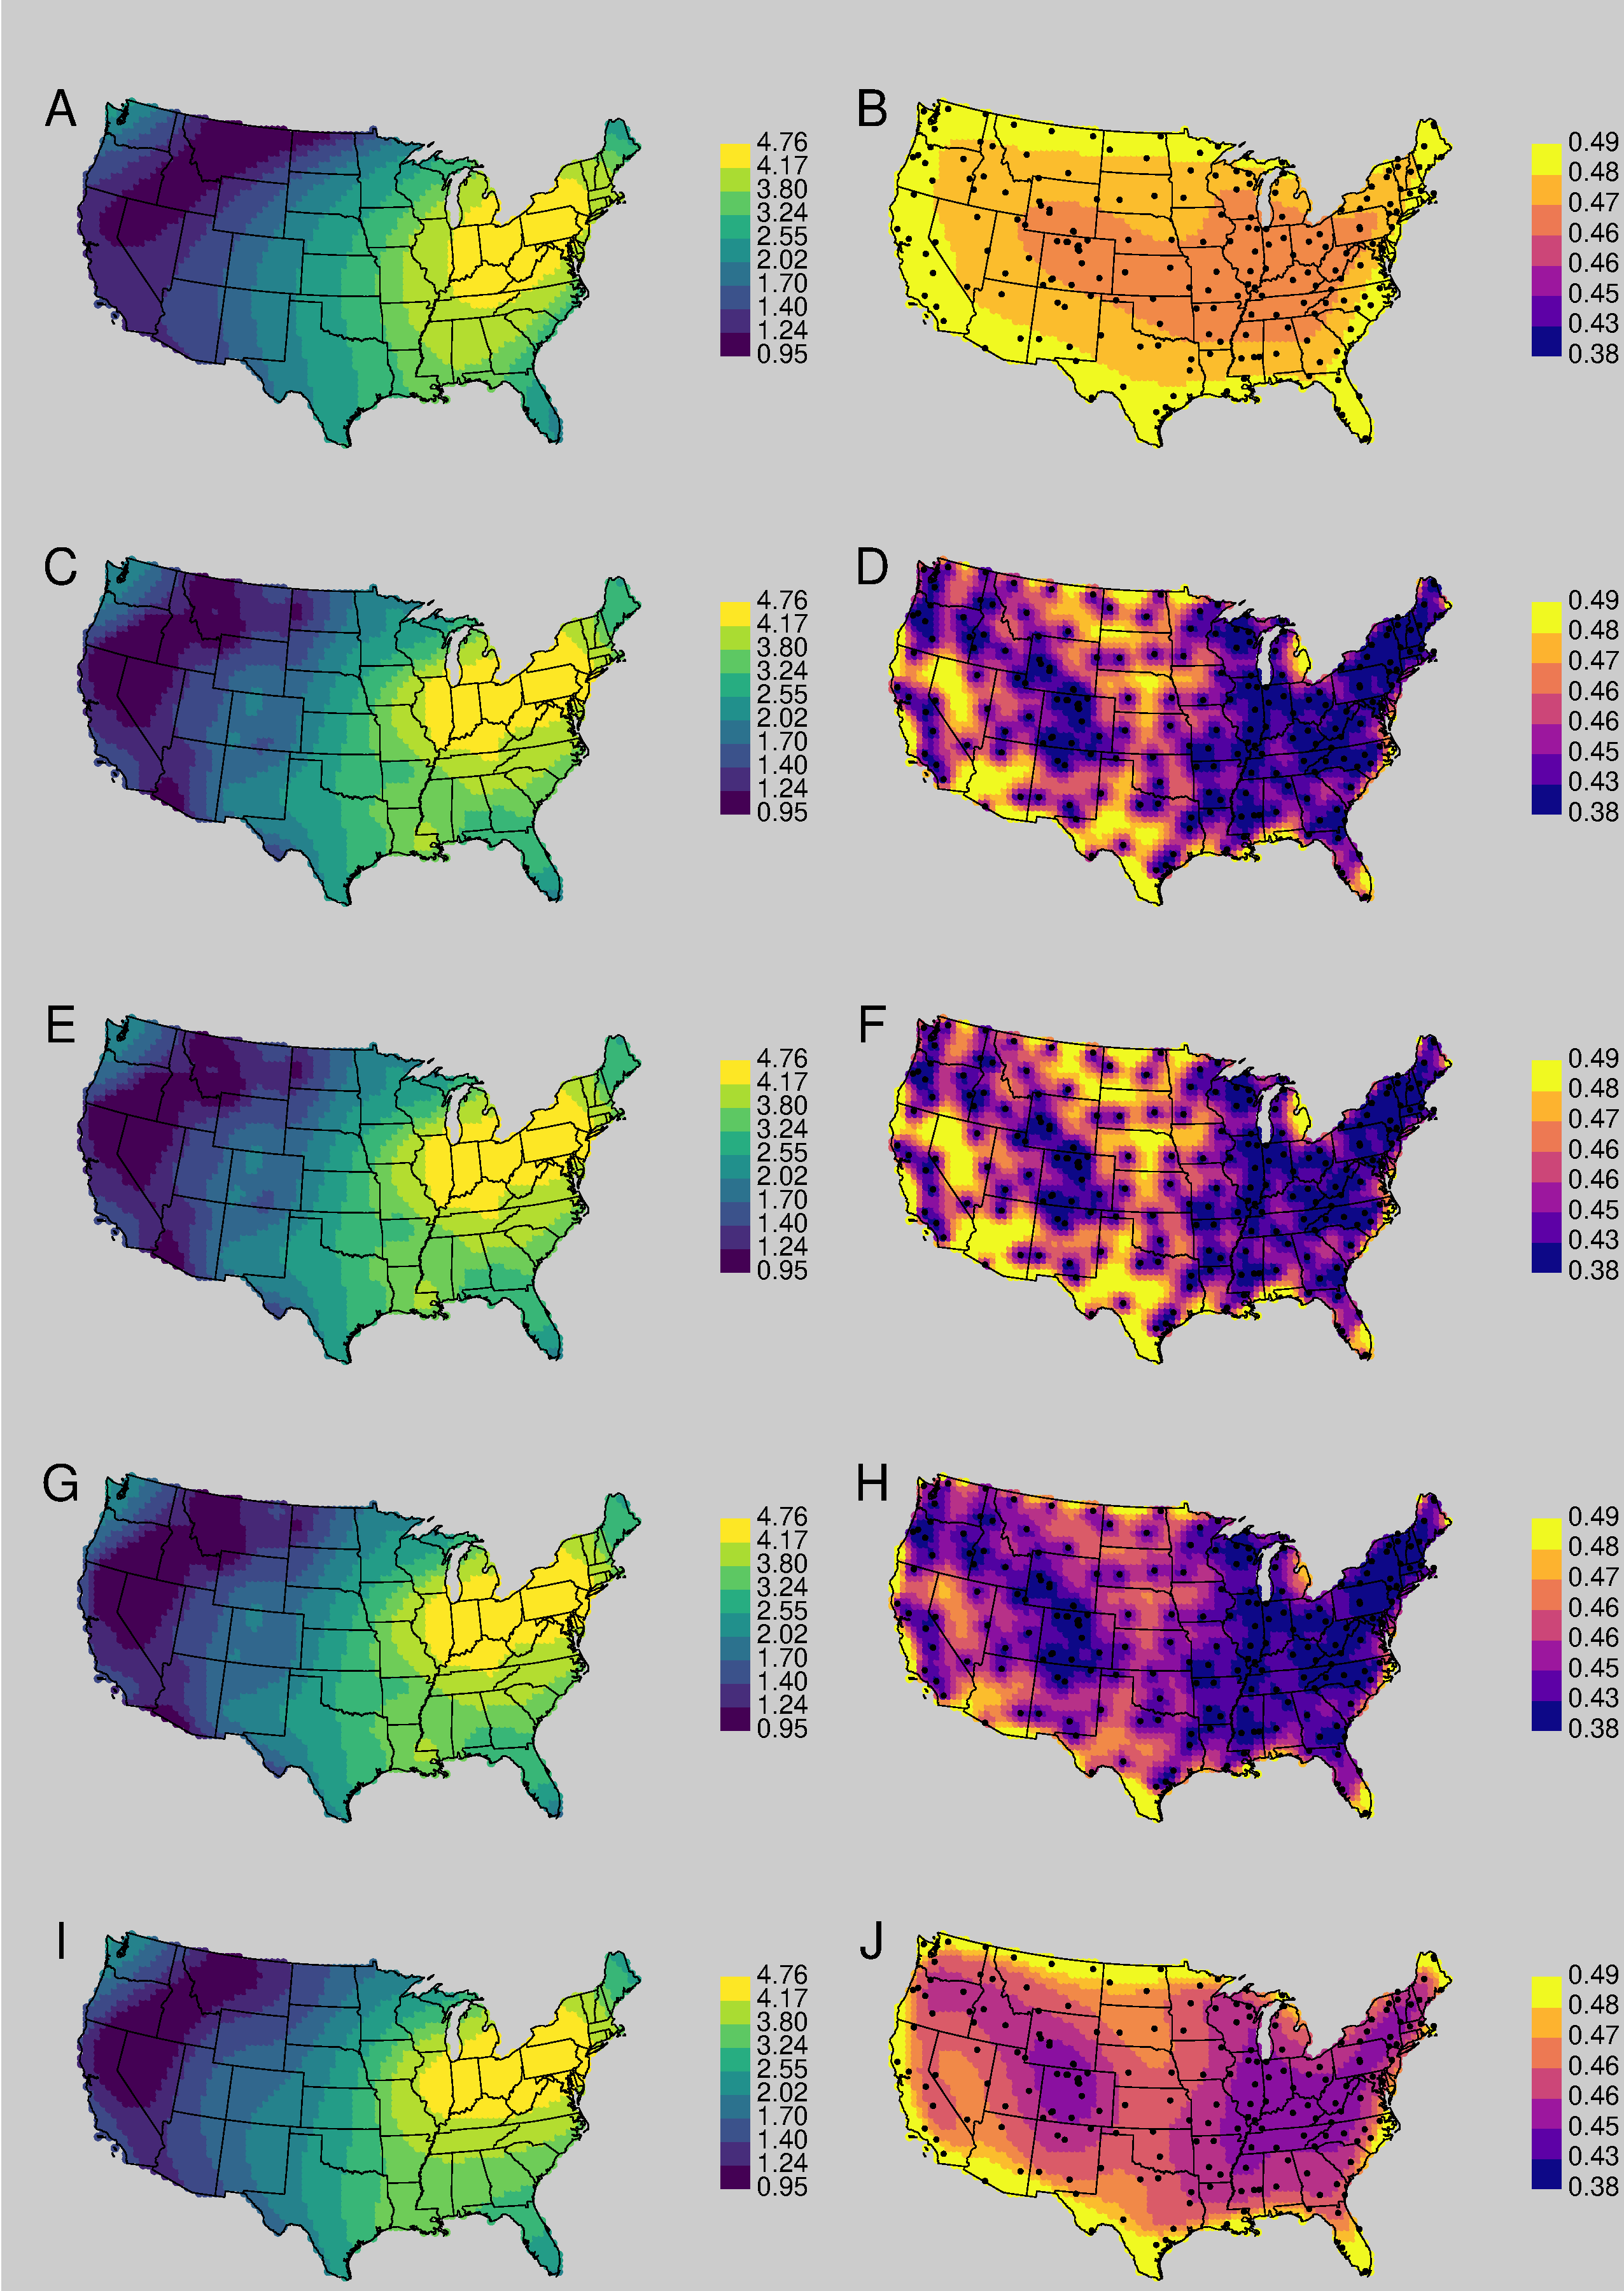
\includegraphics[width=.8\linewidth]{SO4_Prediction_Maps}
  \end{center}
  \caption{Prediction maps (left column) and prediction standard errors (right column) for a variety of models. A-B Fourth-order polynomial assuming independent errors, C-D constant mean spherical model, E-F constant mean exponential model, G-H Third-order polynomial spherical model, I-J constant mean Gaussian model. \label{Fig:SO4_predMaps}}
\end{figure}

%%%%%%%%%%%%%%%%%%%%%%%%%%%%%%%%%%%%%%%%%%%%%%%%%%%%%%%%%%%%%%%%%%%%%%%%%%%%%%%%%%
%%%%%%%%%%%%%%%%%%%%%%%%%%%%%%%%%%%%%%%%%%%%%%%%%%%%%%%%%%%%%%%%%%%%%%%%%%%%%%%%%%
%                BIBLIOGRAPHY
%%%%%%%%%%%%%%%%%%%%%%%%%%%%%%%%%%%%%%%%%%%%%%%%%%%%%%%%%%%%%%%%%%%%%%%%%%%%%%%%%%
%%%%%%%%%%%%%%%%%%%%%%%%%%%%%%%%%%%%%%%%%%%%%%%%%%%%%%%%%%%%%%%%%%%%%%%%%%%%%%%%%%

%\bibliographystyle{consbiol}
\bibliographystyle{/mnt/ExtraDrive1/Work/shTex/asa}
\bibliography{DaleChap883.bib}
%\bibliographystyle{/home/jay/Data/shTex/shTex/asa}
%\bibliography{/home/jay/Data/shTex/shTex/StatBibTex.bib}




\end{document}

